\documentclass[a4paper,twocolumn]{scrreprt}

\usepackage[margin=0.1in]{geometry}

\usepackage[english]{babel}
\usepackage[utf8]{inputenc}

\usepackage{color,xcolor,ucs}

%\usepackage{mathptmx}       % selects Times Roman as basic font
%\usepackage{subfig}
\usepackage{floatrow}
\usepackage{tabularx}
\usepackage{float}
\usepackage{amsfonts}
\usepackage{helvet}         % selects Helvetica as sans-serif font
\usepackage{courier}        % selects Courier as typewriter font
\usepackage{type1cm}        % activate if the above 3 fonts are
% not available on your system
\usepackage{amsmath}
\usepackage{mathtools}
% using for \triangleq
% from http://tex.stackexchange.com/questions/151670/latex-symbol-for-leftrightarrow-with-triangleq
\usepackage{amssymb}
%
\usepackage{makeidx}         % allows index generation
\usepackage{comment}         % allows index generation
\usepackage{graphicx}        % standard LaTeX graphics tool
% when including figure files
\usepackage{epstopdf}
\epstopdfsetup{outdir=./figures/}

\usepackage{multicol}        % used for the two-column index
\usepackage[bottom]{footmisc}% places footnotes at page bottom
\usepackage{bm}

\usepackage{cite}
\usepackage{url}

%\usepackage[bookmarks=true]{hyperref}


\usepackage[unicode=true, bookmarks=true,colorlinks=true]{hyperref}
\usepackage{xr-hyper}


%\newfloat{algorithm}{t}{lop}
%\usepackage[linesnumbered, inoutnumbered]{algorithm2e}
\usepackage{algpseudocode,algorithm,algorithmicx}



\usepackage{xspace}
\usepackage{rotating}

\usepackage{tikz}
%\usepackage{pgfplots}
\usepackage{tkz-graph}
\usetikzlibrary{arrows,shapes,shadows,positioning,calc}


\usepackage{graphicx}
%\graphicspath{{figures/}}

\usepackage{threeparttable}
\usepackage{multirow}
%\usepackage[font=scriptsize,labelfont=bf]{caption}

\usepackage{blkarray}

\usepackage{tikz}
\usetikzlibrary{bayesnet}
\usepackage{subcaption}
\usepackage{verbatim}
\graphicspath{{images/}}

%\usepackage{setspace}
%\usepackage{titlesec}
%\titlespacing*{\section}
%{0pt}{5.5ex plus 1ex minus .2ex}{4.3ex plus .2ex}
%\titlespacing*{\subsection}
%{0pt}{5.5ex plus 1ex minus .2ex}{2.3ex plus .2ex}
\DeclareMathOperator*{\argmin}{arg\,min}
\DeclareMathOperator*{\argmax}{arg\,max}

%\theoremstyle{definition}
\newtheorem{example}{Example}[section]


\definecolor{vadim}{rgb}{1,0.6,0.7}
\definecolor{yuri}{rgb}{0.6,0.6,1}

\definecolor{marker}{rgb}{1,1,0}

\newcommand{\myputtext}[2]{
	\begin{tikzpicture}
	\node [fill=#2, rounded corners=2pt] {#1};
	\end{tikzpicture}
}
%\newcommand{\VI}[1]{\colorbox{vadim}{VI: #1}}
%\newcommand{\YF}[1]{\colorbox{yuri}{YF:#1}}
\newcommand{\VI}[1]{{\color{blue} #1}}
\newcommand{\YF}[1]{{\color{magenta} #1}}


\newcommand{\hl}[1]{\colorbox{marker}{#1}}

\newcommand{\Eqref}[1]{Eq.~(\ref{#1})}
\newcommand{\Figref}[1]{Fig.~\ref{#1}}


\newcommand{\Zeta}{\mathrm{Z}}
\newcommand{\bydef}{\ensuremath{\overset{def}{=}}}
\newcommand{\maxim}[2]{\ensuremath{\underset{#2}{#1}}}
\newcommand{\fnorm}[1]{\ensuremath{{\parallel}#1{\parallel_{\cal F}}}} % this removes spacing, could be ugly for final version


%\DeclarePairedDelimiterX{\nrmB}[2]{\left\lVert}{\right\rVert^2_{#2}}{#1}
\newcommand{\nrm}[2]{\ensuremath{{\parallel}{#2}{\parallel_{#1}}}}
%\newcommand{\nrmsq}[2]{\ensuremath{{\parallel}{#2}{\parallel^2_{#1}}}}
\DeclarePairedDelimiterX{\nrmsq}[2]{\lVert}{\rVert^2_{#1}}{#2}
\newcommand{\expt}[2]{\ensuremath{\underset{{#1}}{\mathbb E}{\{{#2}\}}}}
%\newcommand{\alias}[2]{{#1}\odot{#2}}
\newcommand{\alias}[1]{\ensuremath{\{{#1}\}_{\textbf{aliased}}}}% \xspace}
%\newcommand{\blf}[1]{\ensuremath{b[#1]}}

\newcommand{\prob}[1]{\ensuremath{\mathbb{P}({#1})}}
\newcommand{\blf}[1]{\prob{#1}}


%\usepackage{textcomp,    % for \textlangle and \textrangle macros
%            xspace}
%\newcommand\la{\textlangle\xspace}  % set up short-form macros
%\newcommand\ra{\textrangle\xspace}

%FIXME!
\newcommand\la{\langle\xspace}  % set up short-form macros
\newcommand\ra{\rangle\xspace}

\newcommand*\Let[2]{\State #1 $\gets$ #2}
\algrenewcommand\algorithmicrequire{\textbf{Input:}}
\algrenewcommand\algorithmicensure{\textbf{Input:}}
\algnewcommand{\LineComment}[1]{\State \(\triangleright\) #1}

%new formulation
\newcommand{\priorB}{\ensuremath{\blf{X^-_{k+1}}}\xspace}
\newcommand{\condB}{\blf{X_{k+1} \mid z_{k+1}, \his}\xspace}
\newcommand{\condBi}[1]{\blf{X_{k+1} \mid #1, z_{k+1}, \his}\xspace}
\newcommand{\event}[1]{\ensuremath{A_{#1}}\xspace}

%spaces
\newcommand{\poses}{\ensuremath{{\cal X}}\xspace}
\newcommand{\relpose}{\ensuremath{x^{(rel)}}\xspace}
\newcommand{\relposes}{\ensuremath{{\cal X}^{(rel)}}\xspace}
\newcommand{\observations}{\ensuremath{{\cal Z}}\xspace}
\newcommand{\events}{\ensuremath{\{\event{\mathbb{N}}\}}\xspace}
\newcommand{\controls}{\ensuremath{{\cal U}}\xspace}
\newcommand{\landmarks}{\ensuremath{{\cal L}}\xspace}

\newcommand{\classif}{\ensuremath{{\cal S}}\xspace}
\newcommand{\classes}{\ensuremath{{\cal C}}\xspace}

%history
\newcommand{\his}{\ensuremath{{\cal H}}\xspace}

% history with relative poses
\newcommand{\hisrp}{\ensuremath{{H}}\xspace}

%------------------------------------------------
% Statistical Independence 
% from http://jblevins.org/log/latex-tips
\newcommand\independent{\protect\mathpalette{\protect\independenT}{\perp}}
\def\independenT#1#2{\mathrel{\rlap{$#1#2$}\mkern2mu{#1#2}}}
%------------------------------------------------

%% To select R matrix entries
%\newcommand{\bluex}{\color{blue}\pmb{\times}}
%\newcommand{\redx}{\color{red}\pmb{\times}}

\begin{document}
TO ADD: euler vector to matrix and 
back, inverse of coord system transform, quaternions, transformation 
composition, 3d transformation types, solve bayes specific example, feature 
detection, 
RANSAC
\paragraph*{Probability and Gaussian Identities}
{\tiny
\begin{gather*}
	x\sim N\left(\mu_x, \Sigma_x\right)~y=Ax+b 
	\Longrightarrow \mu_y = A\mu_x + b~\Sigma_y = 
	A\Sigma_x A^T  \\
	\sum_i \nrmsq{\Sigma_i}{A_ix\pm B_i} = 
	\nrmsq[\bigg]{}{\begin{pmatrix}
	\vert \\ \Sigma_i^{-\frac{1}{2}}A_i \\ \vert
	\end{pmatrix}x \pm 
	{\begin{pmatrix}
		\vert \\ \Sigma_i^{-\frac{1}{2}}B_i \\ \vert
		\end{pmatrix}
		}} \\
	I=\sum_i A_i^T\Sigma_i^{-1}A_i, \quad \mu = \mp I^{-1}\cdot \sum_i A_i^T 
		\Sigma_i^{-1}B_i \\
	x\sim N(x;\mu, \Sigma)=	N^{-1}(x; \eta, \Lambda),~ \Lambda \doteq 
	\Sigma^{-1},~ 
	\eta \doteq \Lambda\mu \\
	N^{-1}(x; \eta, \Lambda) = 
		\frac{\exp\left(-\frac{1}{2}\eta^T\Lambda^{-1}\eta\right)}
		{\sqrt{\det\left(2\pi\Lambda^{-1}\right)}} \exp 
		\left(-\frac{1}{2}x^T\Lambda x + \eta^T x\right)
\end{gather*}

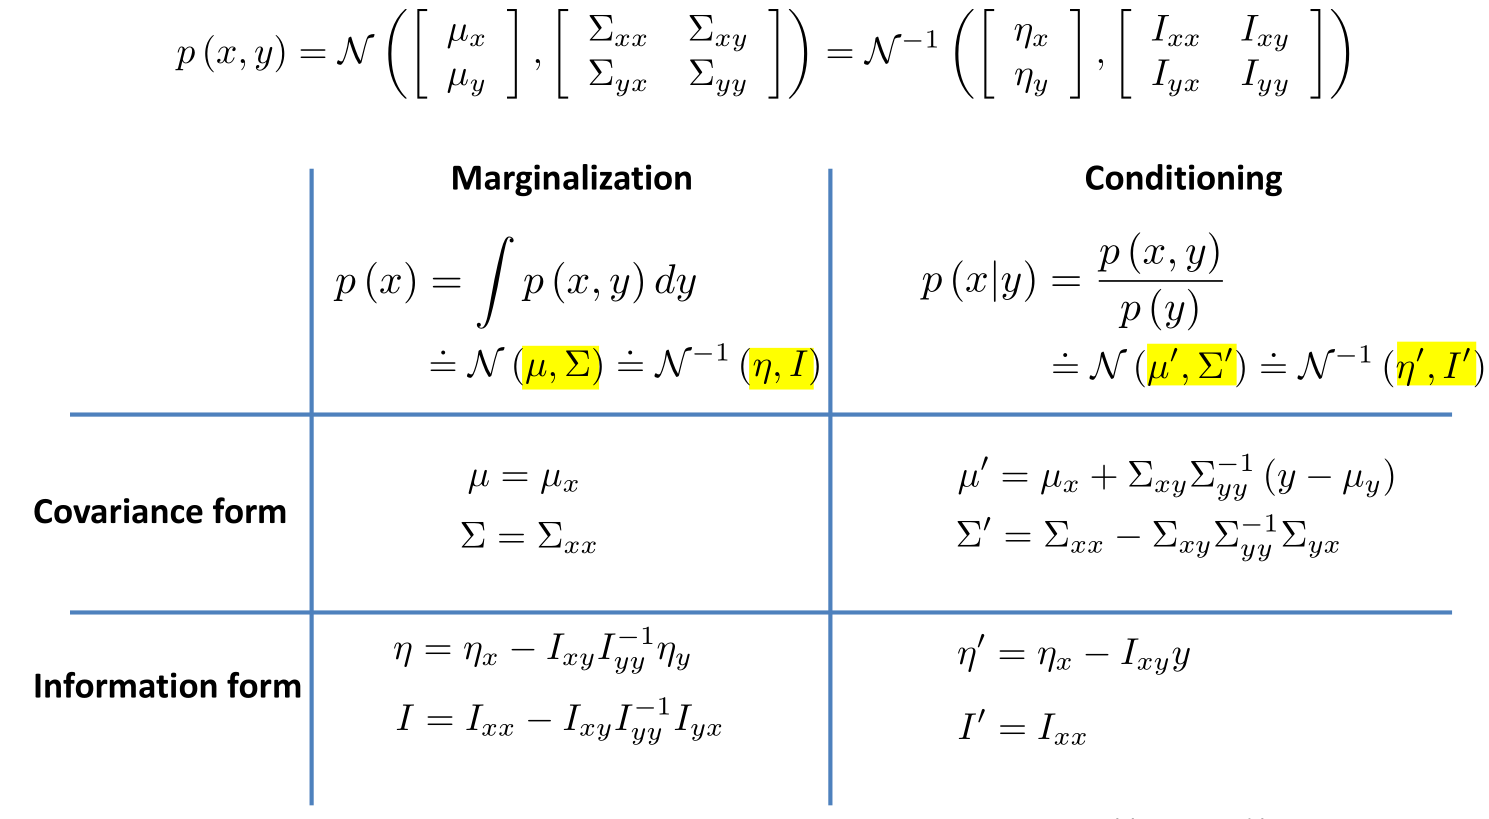
\includegraphics[width=0.8\linewidth]{cond-marg.png} 
}
\paragraph*{Matrix identities}
{\tiny
\begin{gather*}
	[t]_\times \doteq \begin{pmatrix}
	0 & -t_3 & t_2 \\
	t_3 & 0 & -t_1 \\
	-t_2 & t_1 & 0
	\end{pmatrix}, ~ J=\begin{pmatrix}
			\dots & \frac{\partial f_1}{\partial x_i} & \dots  \\
				  & \dots & \\
			\dots & \frac{\partial f_n}{\partial x_i} & \dots 
			\end{pmatrix} = 
			\begin{pmatrix}
			\vert \\ (\nabla f_i)^T \\ \vert
			\end{pmatrix} \\
	\nrmsq{\Sigma}{a} = \nrmsq{}{\Sigma^{-1/2}a},~ \quad \Sigma^{-1} = 
	\Sigma^{-T/2}\Sigma^{-1/2}, ~ A^\dagger = \left(A^TA\right)^{-1} A^T\\
		f(x)=f(x_0) + J (x-x_0)+o(\nrmsq{}{\Delta x}) \\
	\text{SVD: } A = U D V^\ast, ~ \text{columns of $U$, $V$ - ort. 
	eigenvectors of $MM^\ast$ and $M^\ast M$} \\
	\text{QR: } \mathcal{A}\Delta\Theta = \breve{b}, ~ Q^T\mathcal{A} = 
	\begin{bmatrix}
	R \\ 0
	\end{bmatrix}, ~Q^T\breve{b} = \begin{bmatrix}
	d \\ e
	\end{bmatrix}
\end{gather*}
}

\paragraph*{Pose and Geometry}
{\tiny \begin{gather*}
	v^b = R_a^b v_a + t^b_{b\to a} 
	~
	{\tiny\scriptstyle \begin{pmatrix}
	v^b \\ 1
	\end{pmatrix}
	= \begin{pmatrix}
	R_a^b & t^b_{b\to a} \\
	0 & 1
	\end{pmatrix}
	\begin{pmatrix}
	v^a \\ 1
	\end{pmatrix}}
	\\
	T_2T_1 = \begin{pmatrix}
	R_2R_1 & R_2t_1+t_2 \\ 0 & 1
	\end{pmatrix}, ~ T^{-1} = \begin{pmatrix}
	R^T & -R^Tt \\ 0 & 1
	\end{pmatrix}\\
	{\tiny\scriptstyle R_a^b=\begin{pmatrix}
		 &  &  \\
		x_a^b & y_a^b & z_a^b \\
		 &  &  
		\end{pmatrix}=
	\begin{pmatrix}
	x_a\cdot x_b & y_a\cdot x_b & z_a\cdot x_b \\
	x_a\cdot y_b & y_a\cdot y_b & z_a\cdot y_b \\
	x_a\cdot z_b & y_a\cdot z_b & z_a\cdot z_b
	\end{pmatrix}}% 
	\\
	{\tiny {\scriptstyle R_x(\phi) R_y(\theta) R_z(\psi) }= 
	\begin{pmatrix}
		1 & 0 & 0 \\ 
		0 & c_\phi & -s_\phi \\
		0 & s_\phi & c_\phi 
	\end{pmatrix}~
	\begin{pmatrix}
		c_\theta & 0 & s_\theta \\ 
		0 & 1 & 0 \\
		-s_\theta & 0 & c_\theta
	\end{pmatrix}
	\begin{pmatrix}
		c_\psi & -s_\psi & 0 \\ 
		s_\psi & c_\psi & 0 \\
		0 & 0 & 1 
	\end{pmatrix}~
	} \\
	{\scriptstyle\tiny \text{convention: } x^G\doteq \left(R_C^G, t^G_{G\to 
	C}\right)} ~
	{\scriptstyle \text{re-projection error: }
	e = z_{observed}-\pi(x_{true}, l_{true})} \\
	{\tiny\scriptstyle \lambda \begin{pmatrix}
		u \\ v \\ 1
		\end{pmatrix} = 
	\begin{pmatrix}
	\tilde{u} \\ \tilde{v} \\ \tilde{w}
	\end{pmatrix} = K\underbrace{
	\left(\begin{array}{c|c}
	R_G^C & t^C_{C\to G}
	\end{array}\right)}_{M}
	\begin{pmatrix}
	x^G \\ y^G \\ z^G \\ 1
	\end{pmatrix} = 
	M\begin{pmatrix}
		x^G \\ y^G \\ z^G \\ 1
		\end{pmatrix}}, ~ {\tiny\scriptstyle K=\begin{pmatrix}
			\alpha_x & 0 & u_0 \\ 
			0 & \alpha_y & v_0 \\
			0 & 0 & 1
			\end{pmatrix}} \\ 
	{\scriptstyle\tiny u = \frac{m_{11}x + m_{12}y + m_{13}z + 
	m_{14}}{m_{31}x + m_{32}y + m_{33}z + m_{34}} \quad 
	v = \frac{m_{21}x + m_{22}y + m_{23}z + 
		m_{24}}{m_{31}x + m_{32}y + m_{33}z + m_{34}}} \\
	\text{\tiny $a_{x,y} = fk_{x,y}$, $u_0$, $v_0$ - PP in pixels}\hfill
\end{gather*}}
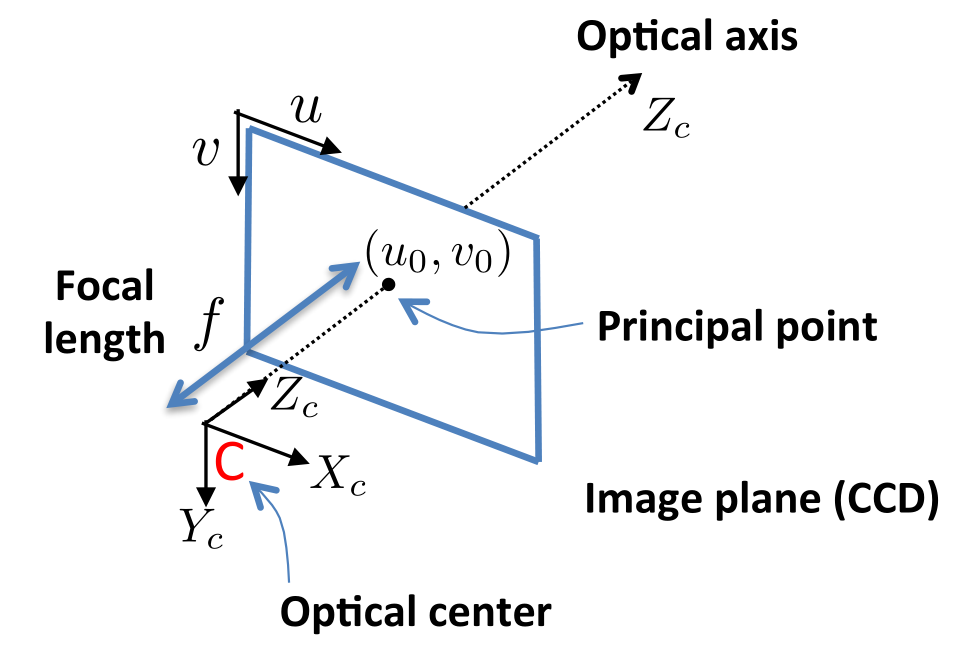
\includegraphics[width=0.4\linewidth]{pinhole.png} 
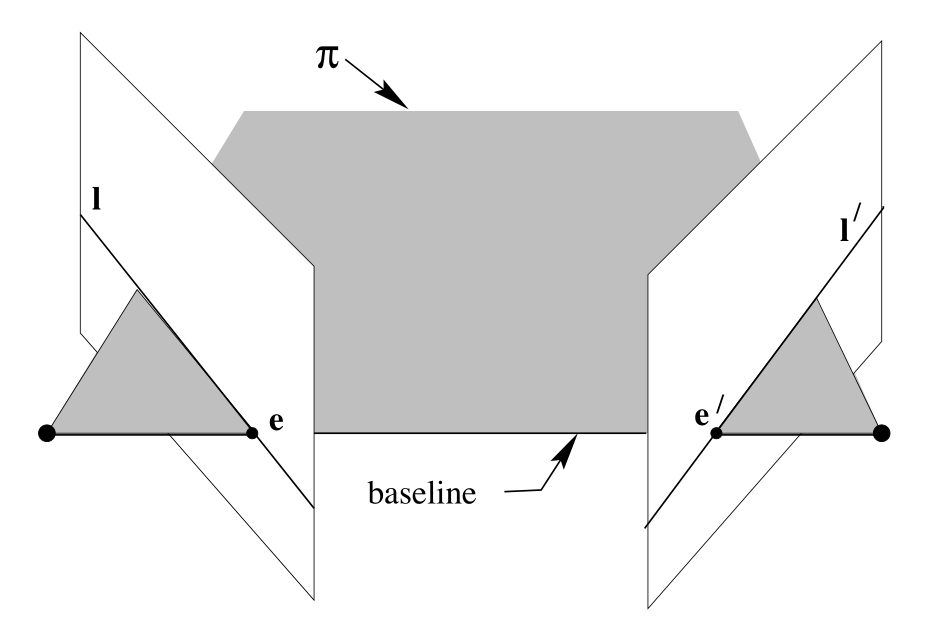
\includegraphics[width=0.4\linewidth]{epipolar.png} 

\paragraph*{Epipolar Geometry}
{\tiny
\begin{gather*}
	q_1\triangleq K_1^{-1}x_1 ~	q_2 \triangleq K_2^{-1}x_2 \quad 
	\text{Epipolar constraint: } q_2^T[t^2_{2\to 1}]_\times R_1^2 q_1 = 0 \\
	\text{Essential M: } E = [t]_\times R \in \mathbb{R}^{3\times 3}~
	\text{Fundamental M: } E = K_2^{ T} F K_1 \\
	\text{F estimation: } 
	\begin{pmatrix}
	x \\ y \\ 1
	\end{pmatrix}^T F
	\begin{pmatrix}
	x^\prime \\ y^\prime \\ 1
	\end{pmatrix} = 0, ~
	\left(x^\prime x, x^\prime y, x^\prime, y^\prime x, y^\prime y, y^\prime, 
	x, y, 1\right) \bm{f} = 0
\end{gather*}

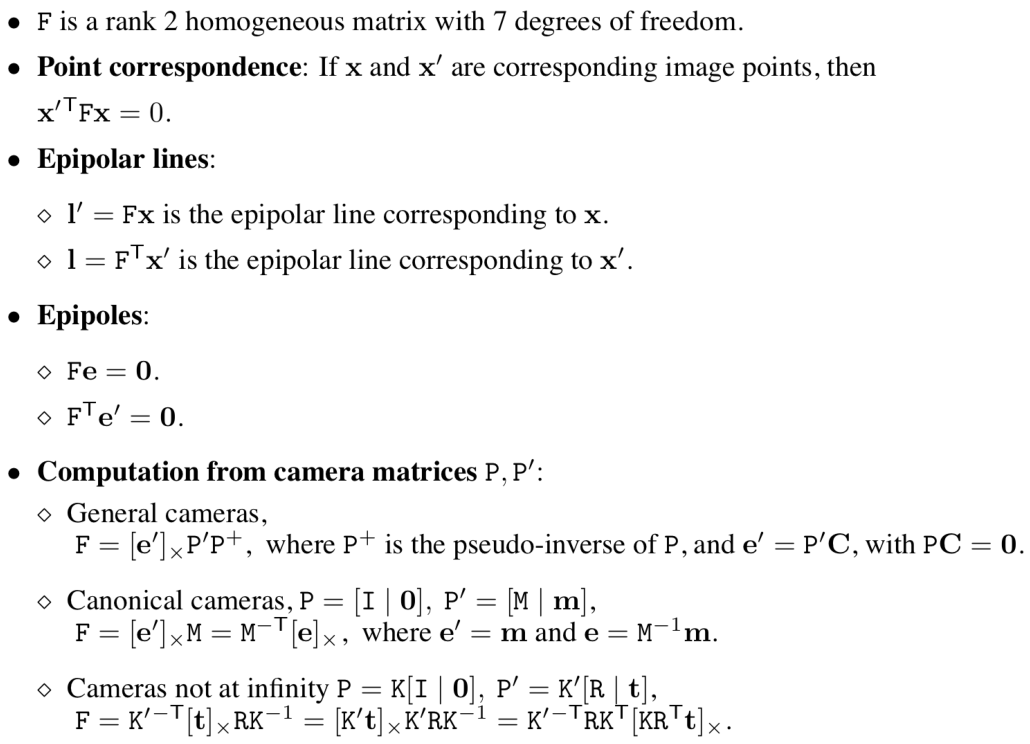
\includegraphics[width=0.8\linewidth]{fundamental.png} 
}

\paragraph*{Kalman Filter}
{\tiny
\begin{gather*}
	x_{k+1} = A_kx_k+B_ku_k+\omega_k, ~ z_k = H_kx_k+v_k \\
%	x_k\in\mathbb{R}^{n\times 1},~u_k\in\mathbb{R}^{p\times 1}, ~ 
%	z_k\in\mathbb{R}^{m\times 1}, ~F_k\in\mathbb{R}^{n\times n}, ~B_k\in 
%	\mathbb{R}^{n\times p}, ~ H_k\in\mathbb{R}^{m\times n}
\end{gather*}
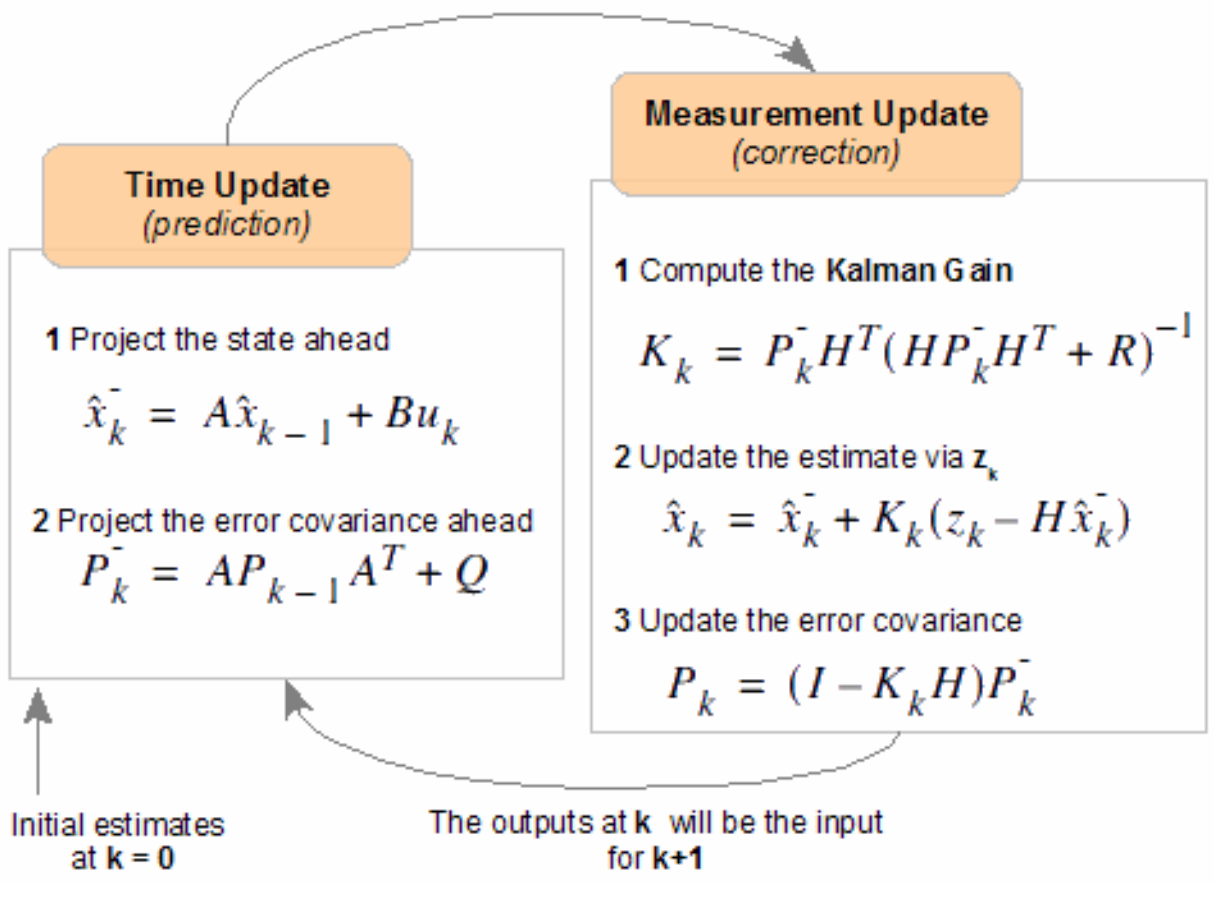
\includegraphics[width=0.7\linewidth]{kalman.png} 
}
\paragraph*{SLAM}
\begin{gather*}
\end{gather*}
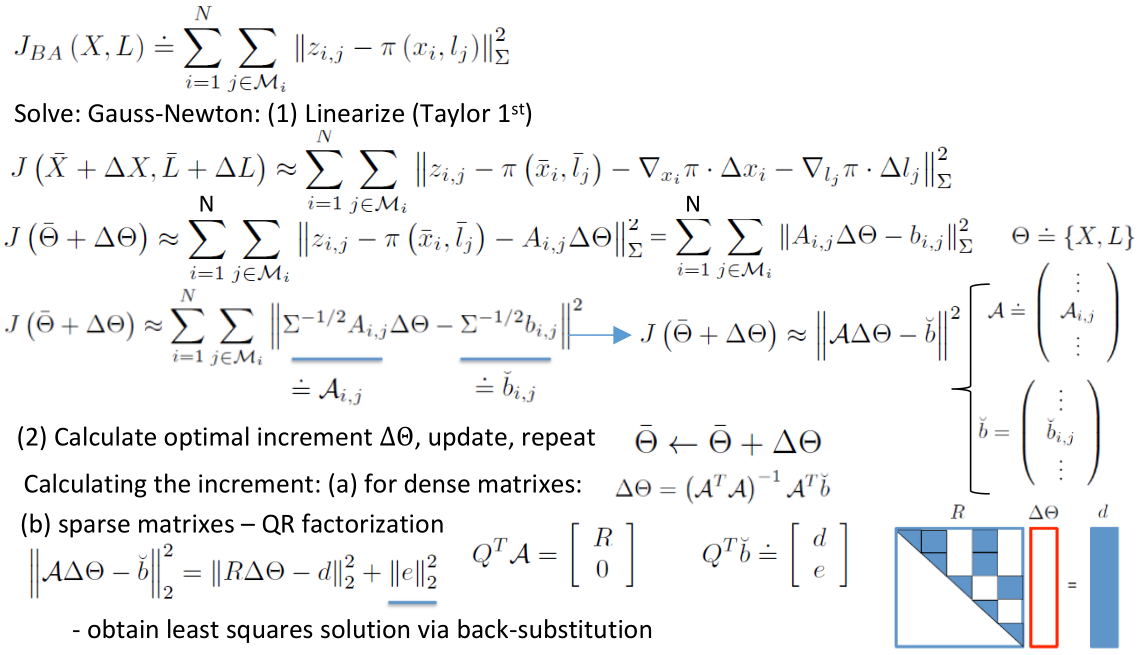
\includegraphics[width=0.8\linewidth]{bundle.png} 
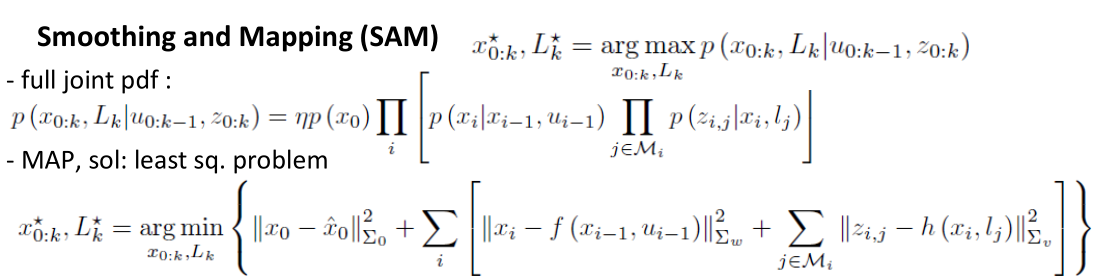
\includegraphics[width=0.8\linewidth]{sam.png} 
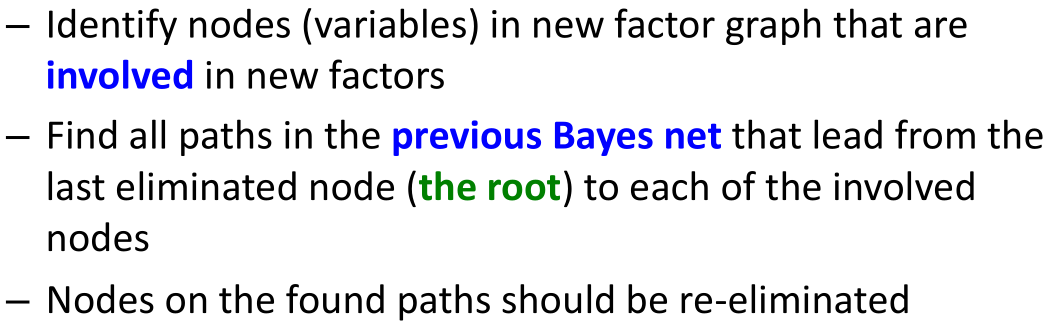
\includegraphics[width=0.6\linewidth]{incremental.png} 


\end{document}
